\section{Related Works}
\label{ch:relate}
\epigraph{If I have seen further it is by standing on the shoulders of Giants.}{Isaac Newton}

% - 讨论 client-side 的 clickstream 为什么值得研究,比较服务端搜集的 clickstream 产生的明显变化是什么。
% - 讨论现有的 client-side clickstream 研究分别是针对什么方向的,他们的结论主要是什么,都有什么样的改进空间。
% - 以前的 clickstream 只有类别级的分配模型,通过人工设计某个特定网站的马尔科夫模型来学习用户在不同类别之间的跳转概率。但当变为客户端后,数据变得更加充分,用户在一段时间内可能不局限于某个特定的网站,同时可能被其他网站干扰。

In this chapter, we discuss the former research that releats to our work, including
the existing approaches to clickstream behavior modeling, the evolution of information 
behavior theory regarding how it adapts to our digital world, as well as the 
most related recent advances regarding sequence learning.

\subsection{Clickstream Behavior Modeling}

Clickstream behavior research can be traced back to the year when the word ``clickstream''
was invented. Eearly clickstream behavior research studied the navigational behavior
of user \cite{mandese1995clickstreams, brodwin1995} and 
they binary classified clickstream based on the degree of linearity.

Mobasher et al. discovered the effective and scalable techniques \cite{Mobasher:2001:EPB:502932.502935} for Web personalization
by using association rules and built a recommondation system. Goldfrab invistigates \cite{goldfarb2002analyzing} 
the website choice behavior based on clickstream data and suggests that clickstream simulate company strategy changes.
Afterwards, 
Chatterjee et al. \cite{chatterjee2003modeling} first conduct 
the previous research regarding clickstream to an actual commercial website.
They found that clickstream represents an implication that dynamic advertising
based on customer clickstream history influence the future clickstream of the customer
and increase the interaction with the dynamic advertisement.
More techniquely, Ting et al. uses common sequences to find unexpected browsing behavior \cite{Ting:2005:UMF:1092358.1092469},
and then use their findings to improve website design. 

The most recent research evolved the approach of clickstream modeling,
Wang et al.\cite{Wang:2016:UCC:2858036.2858107} proposed a unsupervised appraoch to model clickstream without labeling.
Chi et al. proposed an analysis framework \cite{chi2017towards} for the general understanding of online information behavior
in a specific page. However, their framework only fits for server side collected clickstream other than a real user clickstream.
Then, Wang et al. \cite{Wang:2017:CUB:3127338.3068332} improved their unsupervised appraoch,
and summarized more approaches for clickstream behavior modeling that identifies span ad abuse
for a specific website. Park et al. models and detects a behavior change among student while learning 
based on Poisson process \cite{Park:2017:DCS:3027385.3027430} to
help improve online learning experience. Amo et al. \cite{amo2018learning} further visualizes search-stream
behavior based on student clickstream on a class, and Shimada et al. proves \cite{Shimada:2018:OCD:3170358.3170412}
online change detection while monitoring on student behavior is possible based on a sliding window.

Zaloudek gives an review on the comparasion \cite{mastersthesis} traditional method to model clickstream data,
then proposed a principle component analysis based method for a semi-supervised learning
of clickstream data, however their approach does not work well on clustering task, and 
the best performance is obtained by traditional multilayer perceptron algorithm.
Chandramohan and Ravindran then further investigate the neural approach on clicksteam mining \cite{N:2018:NAB:3152494.3152505},
they verified that complexy LSTM with Attention mechanism is able to capture whether a user
is intent to buy a product or not based on server side collected clickstream.
Surprisingly, Gundala and Spezzano \cite{Gundala:2018:RDH:3184558.3191644} simply use a Lasso
regression based on sofisticated feature engineering 
archived AOC score 0.769 for reader demand hyperlink prediction on Wikipedia clickstream dataset.

Kammenhuber et al. is the first study regarding client side clickstream \cite{Kammenhuber:2006:WSC:1177080.1177110}.
They proposed a finite-state Markov model that models user's search behavior on a level of
topic categories. Unfortunately their dataset are collected from network package traffic,
and did not consider the time a user spend in each page.


% 关于 assistent 的研究
% @article{lieberman1995letizia,
%   title={Letizia: An agent that assists web browsing},
%   author={Lieberman, Henry and others},
%   journal={IJCAI (1)},
%   volume={1995},
%   pages={924--929},
%   year={1995}
% }

\begin{figure}[H]
    \centering
    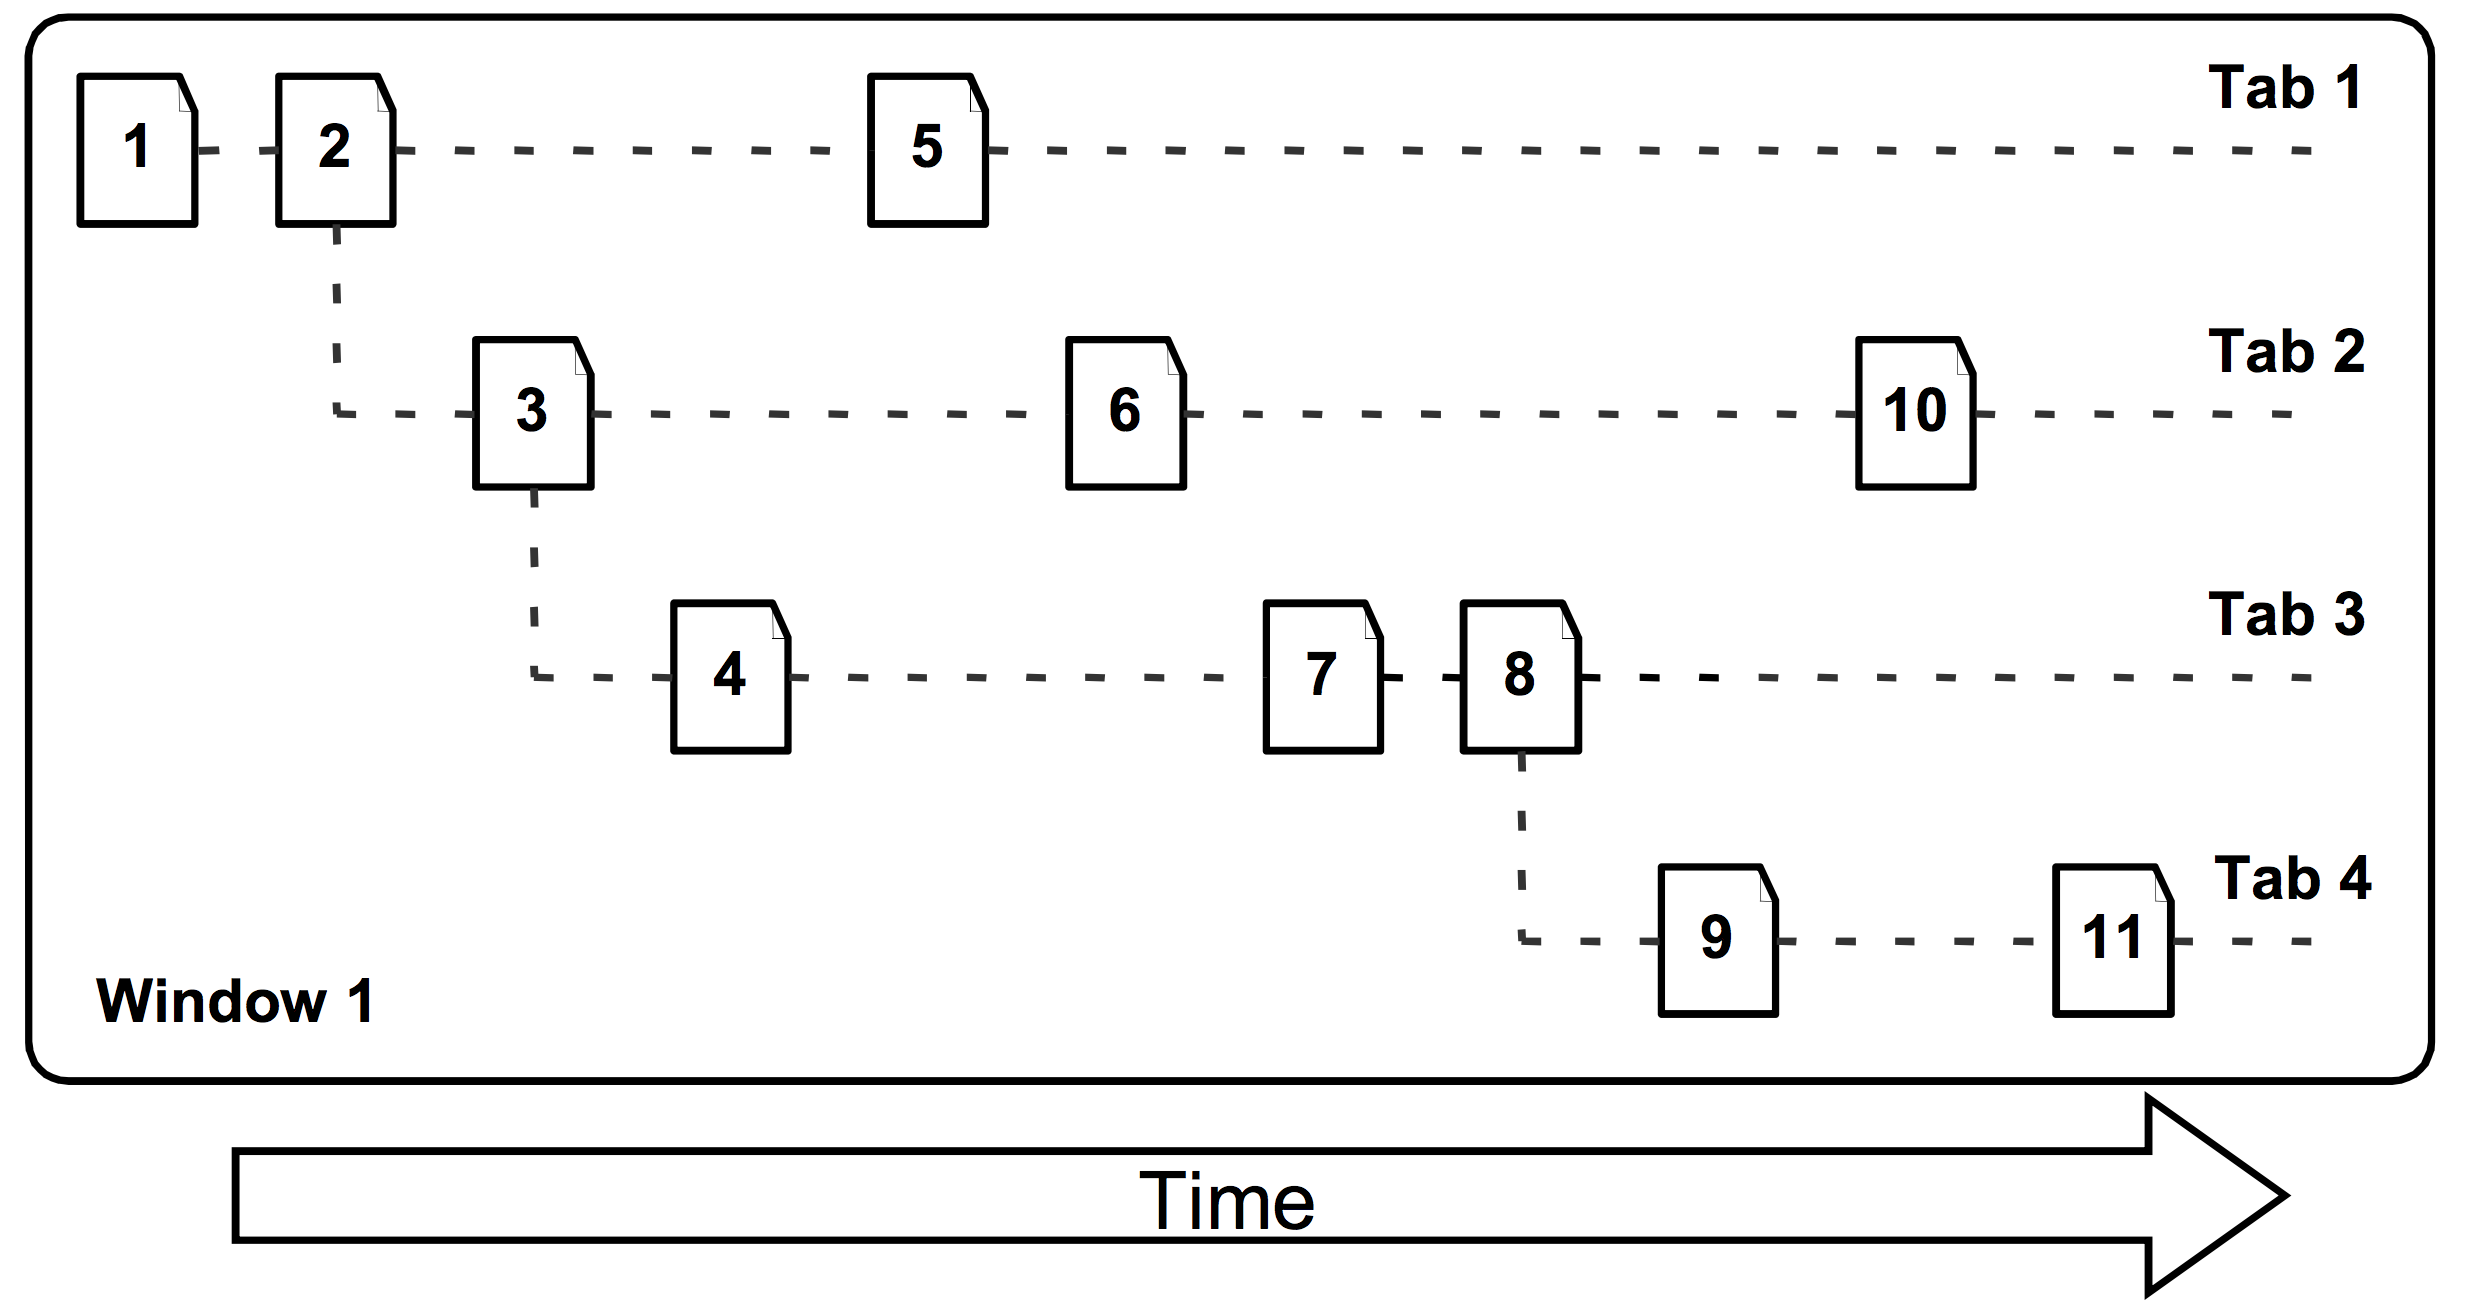
\includegraphics[width=0.55\textwidth]{figures/branching-and-backtracking}
    \caption{Parallel browsing behavior: branching phenomenon \cite{huang2010parallel}}
    \label{fig:backtrace}
\end{figure}

Liu et al. \cite{liu2010understanding} studied a specific user behavior on dwell time on web pages, and concluded that
Weibull distribution is the most appropriate distribution to characterize this behavior. 
Huang et al. \cite{huang2010parallel, huang2012no} further 
noticed the behavior of branching parallel browssing and backtracking browsing
behavior on modern browsers, as shown in Figure \ref{fig:backtrace}, 
and presented an frequent analysis for the distribution of these two behavior individually.

Unfortunately, as we discussed above, the existed research regarding clickstream 
behavior modeling are either server-side modeling for an individual client or 
individually modelized for client-side behaviors with limited information of clickstream,
which does not stands for a real user behavior. 
Besides, the existed approaches are based on self-constructed features, 
the property of Markov memoryless and etc. Though the most recent
approach use neural networks, their findings only applies to specific context.

From the point of view of user behavior, they 
neither unambiguously justifies the foundation of their model, 
nor providing a significative performance of their model.

We, in this thesis, serialize the client side chronologic URL sequences with combines all 
these individually studied phenomena including the branching and backtracking browser 
feature. With this chronologic URLs, we seek to model and understand the essential user 
behaviors patterns while browsing on the Web.

\subsection{Theory of Information Behavior on the Web}
\label{sec:info-seek}

The thesis relates to information behavior theory since it supports the foundation of our
user study. This subsection discusses how the theory was concluded and 
the principles of the theory that sustain our thesis.

Information behavior research encompasses intentional information seeking and 
unintentional information encounters, and the roots to information behavior 
theory relates to information needs and uses \cite{doi:10.1002/aris.2009.1440430114} 
that arose in the 1960s.

However, the concept of information seeking behavior, was coined in late 1981 
by Thomas Wilson \cite{wilson1981user}, and he tries to formalize the process or 
activities of a conscious effort while information needs 
and uses. Figure \ref{fig:wilson-info-seek} illustrate the model of information behavior 
was proposed.

\begin{figure}[H]
    \centering
    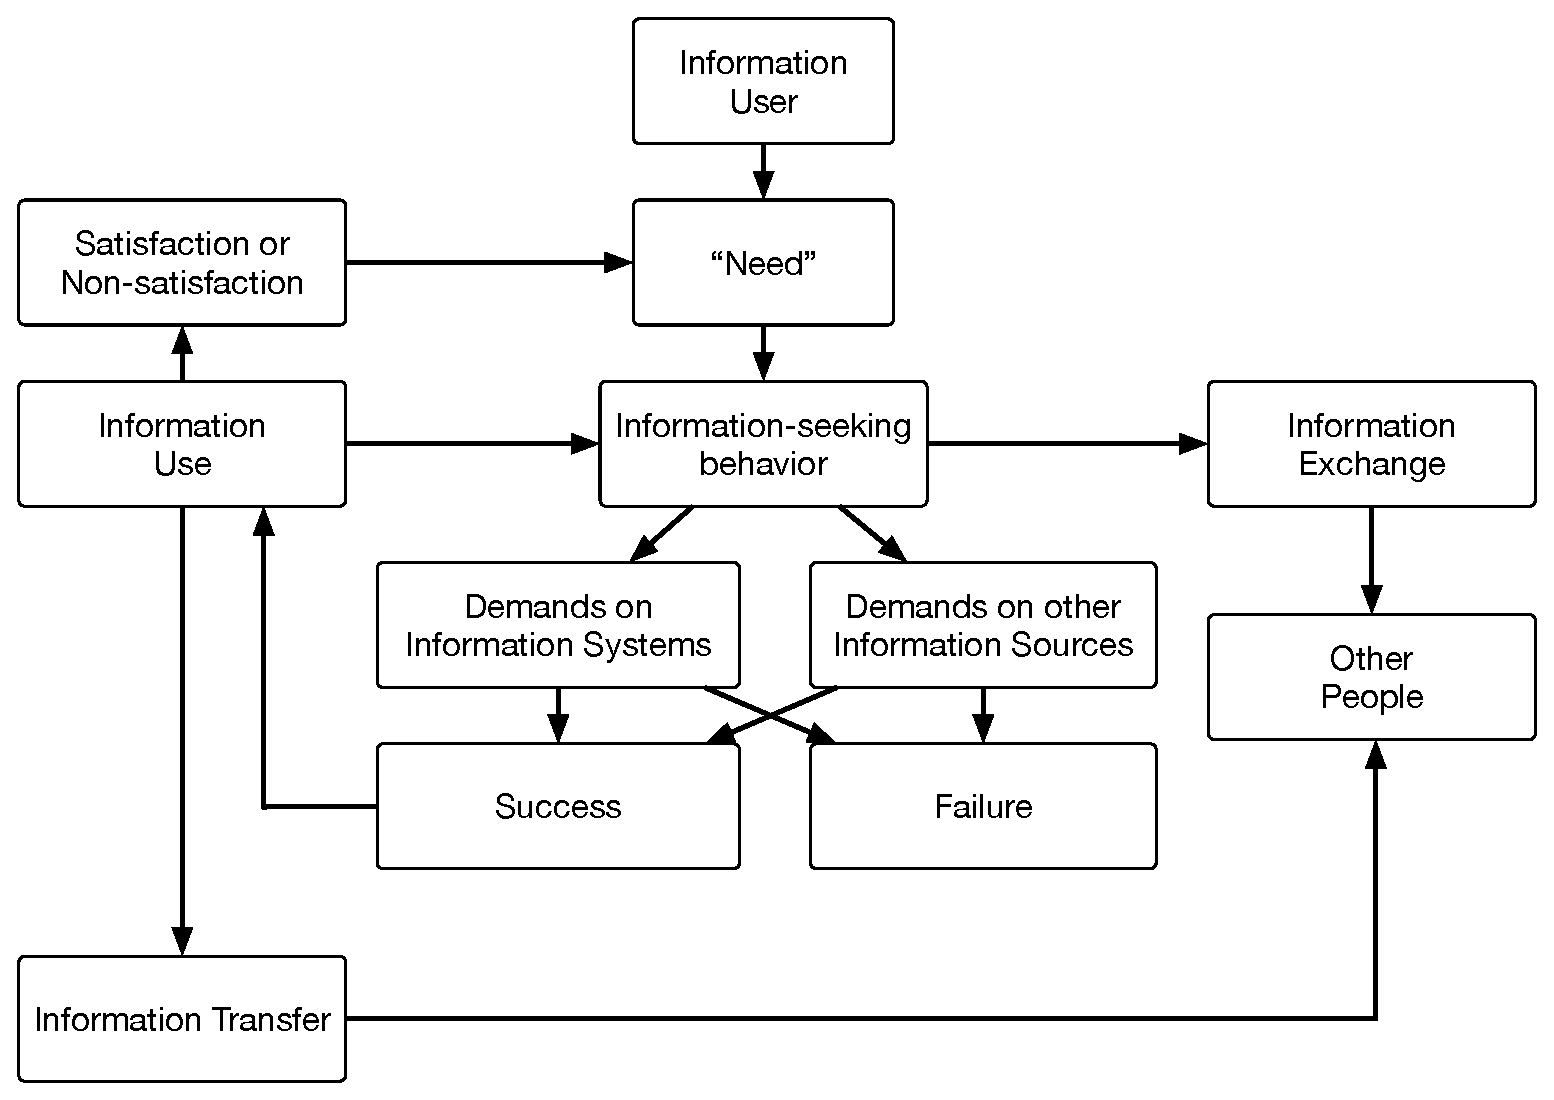
\includegraphics[width=0.7\textwidth]{figures/wilson-info-behavior}
    \caption{Wilson's information seeking behavior model \cite{wilson1981user}}
    \label{fig:wilson-info-seek}
\end{figure}

Wilson's model has been envolved many years since its origin, and it was revised 
and adapted to our digital world since the digital systems learns user preferences and 
changes \cite{giannini1998receiving} the way we receiving information.

David Ellis described a detailed group of activities for information seeking behavior \cite{ellis1989behavioural},
and then applied in physical and social science \cite{ellis1993comparison} and industrial
environment \cite{ellis1997modelling}.
In addition, his analysis was
based on grounded theory approach \cite{aceto1994grounded} and semi-structured interviews. 

Afterwards, Choo et al. adapts Ellis' Model and discussed \cite{choo1999information}
the information seeking behavior on the web through different activities rather 
than a single process, the applied activities are:
starting, chaining, browsing, differentiating, monitoring, and extracting.

``\emph{Starting}'' on the web indicates that a user identifies websites or pages
that containing the information of interests.
``\emph{Chaining}'' indicates that a user follows on starting page to other related pages.
``\emph{Browsing}'' then represents the activity that a user only skimming on the web
and quickly viewing the top-level informations. The ``\emph{differentiating}'' 
describes that a user on the web is selecting useful pages and choosing differentiated.
``\emph{Monitoring}'' activity is used for receiving updates on the sites, or revisit
the previously visited pages. Finally ``\emph{extracting}'' is the activity that a user
systematically extracts informations from a interested page or website.

By applying these activities, Choo et al concludes general user behaviors on the web are
undirected viewing, conditioned viewing, informal search and formal search.
Johnson further describes \cite{johnson2017patterns} seven more detailed behaviors 
patterns on the web, but did not given a working study that verify or prove their formation.

Although Wilson's model and Ellis' model are revised in recent works, however these improvements
are more generic and too complexy for describing user information behavior on the web.
Therefore, in this thesis, we only uses the an antecessor of Wilson's framework \cite{wilson1997information} and 
Ellis' model \cite{ellis1997modelling} to formalize and justify our lab study experiment later in Chapter \ref{ch:exp}, 
as a fundation of our work.

\subsection{Theory of Sequence to Sequence Learning}
\label{sec:seq-learn}

Sequence learning is a large scope of research and has been applied to many fields such as 
machine translation. In machine translation, a series of words are considered as a sequence of
vectors, neural network based models considered representation learning of nature languages.
The initial vectors of word were one-hot encoded vectors and get updated over training and learning.

The recent advances of representation learning uses a distributed representation 
of word2vec model \cite{DBLP:journals/corr/abs-1301-3781}, which achieve better 
performance in natural language processing. The word2vec model introduced 
continous bag-of-word and skip-gram model as an efficient method for learning high-quality
vector representation of words, and bag-of-word is faster while skip-gram is slower but get better
performance for infrequent words.

\cleardoublepage